% ex: tw=74 ts=2 sw=2 noet sts=2
\documentclass[10pt]{report}
\usepackage[utf8]{inputenc}
\usepackage{amsmath}
\usepackage{xkeyval}
\usepackage[bookmarksnumbered,frenchlinks]{hyperref}
%\hypersetup{pdfborder=0 0 0}
\usepackage{multirow}
\usepackage[english]{babel}
\usepackage{fullpage}
\usepackage{tabulary}
\usepackage{tabularx}
%\usepackage{natbib}
\usepackage[all]{hypcap}
\usepackage{hyperref}
\usepackage{framed}
\usepackage{fullpage}
\usepackage{graphicx}
\usepackage{listings}
\usepackage{subfig}
\usepackage{float}
%\floatstyle{boxed} 
%\restylefloat{figure}
\title{\textbf{Experiment 1} \\
	Activity 2}
\author{Cody Schafer}
\date{\today}
\begin{document}
\maketitle
\section{Introduction}
% An Introduction containing a brief description of the lab

	This lab will familiarize you with the voltage transfer
	characteristics and switching times of a BJT inverter.  There are
	two different activities.  In the first activity you will look at
	the operation of a diode and the capacitances at the p-n junction.
	In the second, the operation of a BJT inverter circuit, and
	different ways to eliminate delays in input response will be
	explored.    

\section{Activites}
% A description of each activity and what was accomplished

	In the second activity (activity 1 was completed in lab 1),
	iverters were constructed using a bjt an a resistor. Various
	properities of this circuit were noted, and then, to decrease the
	storage times, the addition of a diode and then the addition of a
	capacitor to the circuit was tested.

\section{Data}
% Any data, tables, or graphs developed in the course of the lab

	\subsection{Determination of Saturation Voltage}

	See Anthony's portion of the report for this section.

	5V was attached to $V_{cc}$ and $V_i$ was varied from 0 upward by
	incriments of 0.2V until the transistor turned on.

	\begin{table}[H]
		\centering
		\subfloat[TIP31 transistor data]{
			\begin{tabular}{c|c|c}
				$V_i$ & $V_{BE}$ & $V_o$ / $V_{CE}$ \\ \hline
				0.0	& 0.010 & 5.060 \\
				0.2	& 0.212	& 5.061 \\
				0.4 & 0.414 & 5.061 \\
				0.6 & 0.58	& 4.375 \\
				0.8	& 0.627 & 0.813 \\
				1.0	& 0.634	& 0.087 \\
				1.2 & 0.636 & 0.067 \\
				1.4 & 0.639 & 0.056 \\
				1.6 & 0.641 & 0.048 \\
				1.8 & 0.644 & 0.043
			\end{tabular}
		}
		\qquad
		\subfloat[2N3904 transistor data]{
			\begin{tabular}{c|c|c}
				$V_i$ & $V_{BE}$ & $V_o$ / $V_{CE}$ \\ \hline
				0.0	& 0.012 & 5.067 \\
				0.2	& 0.213	& 5.067 \\
				0.4 & 0.414 & 5.067 \\
				0.6 & 0.614	& 5.041 \\
				0.8	& 0.706 & 2.123 \\
				1.0	& 0.760	& 0.170 \\
				1.2 & 0.762 & 0.140 \\
				1.4 & 0.763 & 0.126 \\
				1.6 & 0.765 & 0.117 \\
				1.8 & 0.766 & 0.111 \\
				2.0 & 0.767 & 0.106 \\
				2.2 & 0.769 & 0.101 \\
				2.4 & 0.770 & 0.098 \\
				2.6 & 0.770 & 0.095 \\
				2.8 & 0.771 & 0.092 \\
				3.0 & 0.772 & 0.090
			\end{tabular}
		}

		\caption{Data recorded from raising the $V_i$ in 0.2V inciments.}
		\label{tbl:1}
	\end{table}

	\subsection{Second Part}
	See Anthony's report for this section.

	\subsection{Third Part}
		\begin{center} \begin{tabular}{*{6}{c|}c}
			Transistor & $V_{OH}$ & $V_{OL}$ & $t_{d1}$ & $t_f$ & $t_s$ & $t_p$
			\\ \hline

			TIP31 & 5.08 & 0.320 & 197ns & 549ns & 0 & 3.49us \\

			2N3904 & 5 & 0.440 & 58.7ns & 421ns & 0 & 2.57us \\

		\end{tabular} \end{center}

		\begin{figure} \begin{center}
			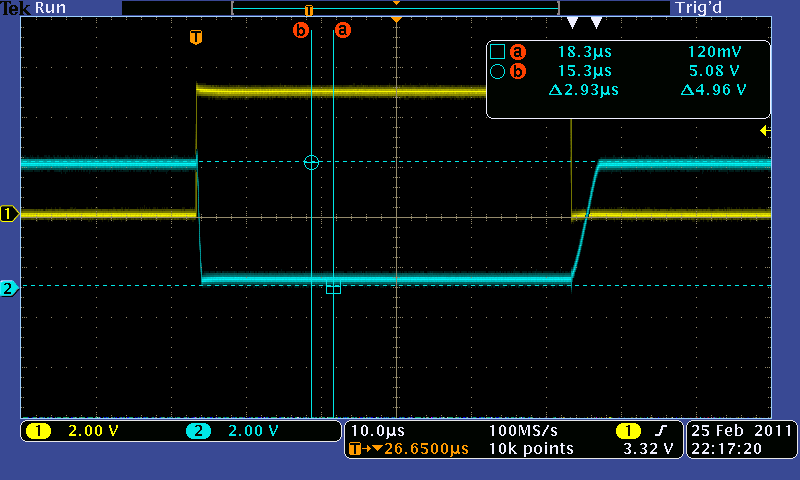
\includegraphics[width=4.5in]{wave_3_tip31.png}
			\caption{TIP31 Wave with diode inserted}
		\end{center} \end{figure}

		\begin{figure} \begin{center}
			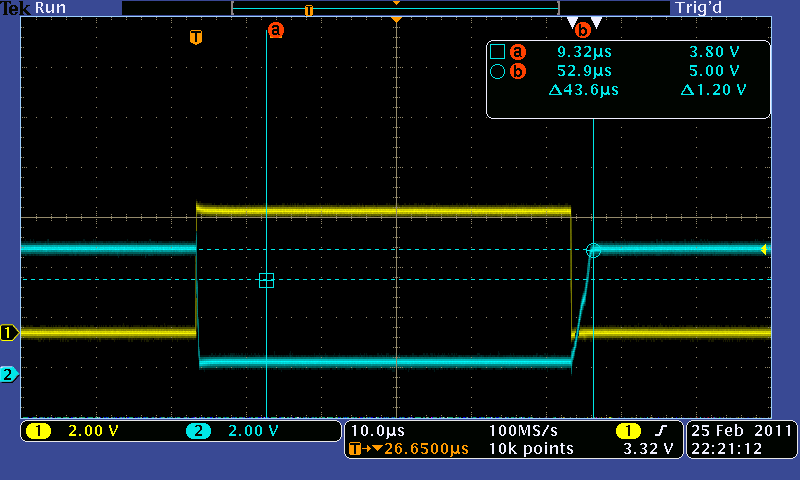
\includegraphics[width=4.5in]{wave_3_3904.png}
			\caption{2N3904 Wave with diode inserted}
		\end{center} \end{figure}


	\subsection{Fourth Part}
		\begin{center} \begin{tabular}{*{4}{c|}c}
			Transistor & $T_d$ & $T_f$ & $T_s$ & $T_r$ \\ \hline

			TIM31 & 53.3ns & 20.0ns & 2.63us & 181ns \\
			2N3904 & 29.3ns & 17.3ns & 0 & 151ns \\
		\end{tabular} \end{center}
		
		\begin{figure}[H]
			\subfloat{
				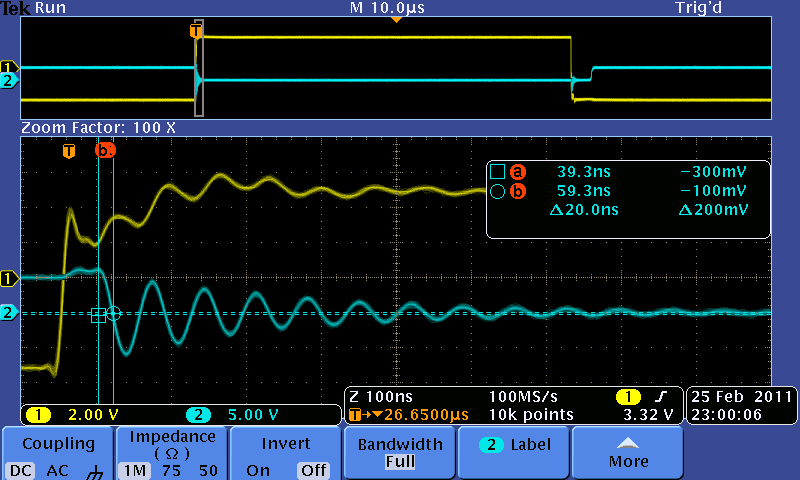
\includegraphics[width=3.2in]{wave_4_tip31_a.png}
			}
			\subfloat{
				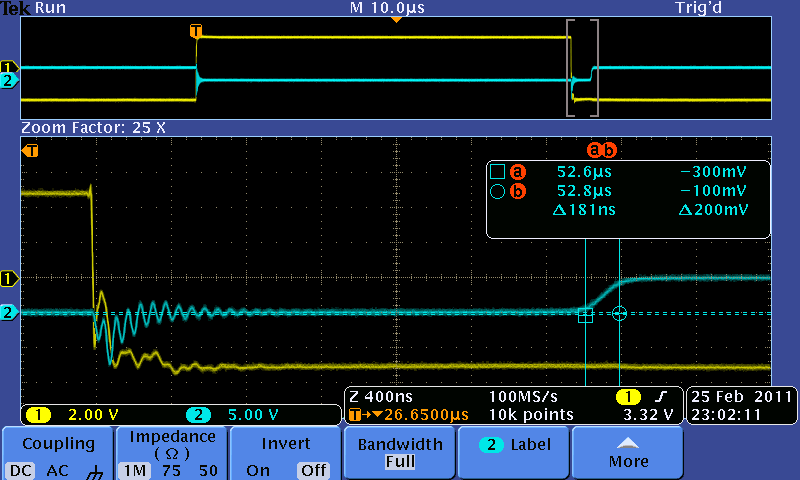
\includegraphics[width=3.2in]{wave_4_tip31_b.png}
			}
			\caption{TIP31 Wave with capacitor inserted}
		\end{figure}

		\begin{figure}[H]
			\subfloat{
				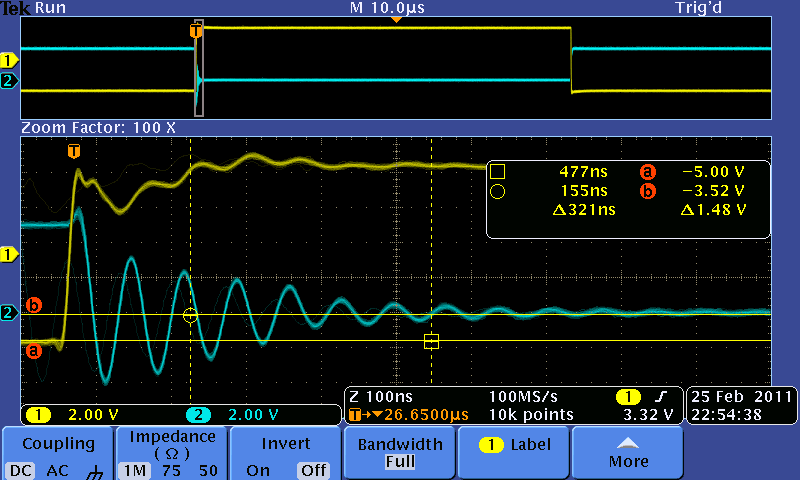
\includegraphics[width=3.2in]{wave_4_3904_a.png}
			}
			\subfloat{
				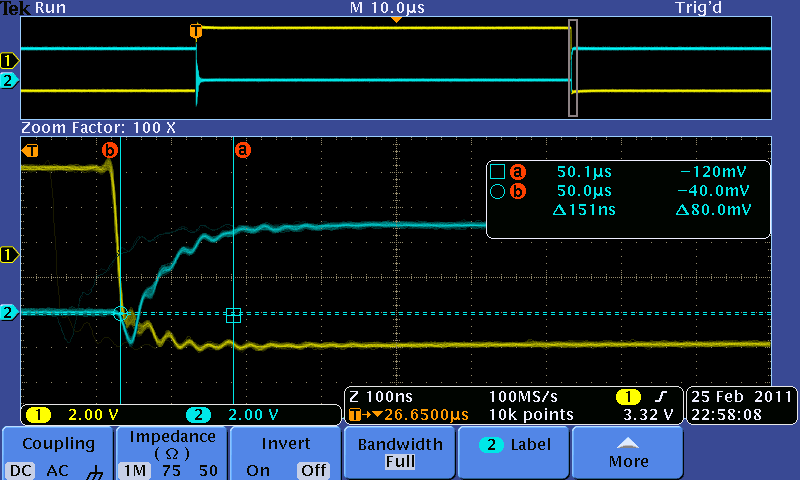
\includegraphics[width=3.2in]{wave_4_3904_b.png}
			}
			\caption{2N3904 Wave with capacitor inserted}
		\end{figure}


\section{Discussion}

\subsection{DC analysis of the Inverter}

\subsection{AC analysis of the Inverter}

\subsection{Inverter with diode clamping}

\subsection{Inverter with added capacitor}


% The SPICE simulation (the prelab)
%
\begin{figure}[H]
	\centering
	\includegraphics[width=4.5in]{p1.eps}
	\caption{Problem 1}
	\label{fig:1}
\end{figure}

\begin{framed}
	\lstinputlisting{p1.spice}
\end{framed}


\begin{figure}[H]
	\centering
	\includegraphics[width=4.5in]{p2.eps}
	\caption{Problem 2}
	\label{fig:2}
\end{figure}

\begin{framed}
	\lstinputlisting{p2.spice}
\end{framed}


\begin{figure}[H]
	\centering
	\includegraphics[width=4.5in]{p3.eps}
	\caption{Problem 3}
	\label{fig:3}
\end{figure}

\begin{framed}
	\lstinputlisting{p3.spice}
\end{framed}


\begin{figure}[H]
	\centering
	\includegraphics[width=4.5in]{p4.eps}
	\caption{Problem 4}
	\label{fig:4}
\end{figure}

\begin{framed}
	\lstinputlisting{p4.spice}
\end{framed}


\begin{figure}[H]
	\centering
	\includegraphics[width=4.5in]{p5.eps}
	\caption{Problem 5}
	\label{fig:5}
\end{figure}

\begin{framed}
	\lstinputlisting{p5.spice}
\end{framed}


\begin{figure}[H]
	\centering
	\includegraphics[width=4.5in]{p6.eps}
	\caption{Problem 6}
	\label{fig:6}
\end{figure}

\begin{framed}
	\lstinputlisting{p6.spice}
\end{framed}



\end{document}
